\documentclass[aspectratio=169,11pt]{beamer}
\usepackage[T1]{fontenc}
\usepackage{lmodern,booktabs,graphicx,tikz}
\usetikzlibrary{arrows.meta,positioning}
\definecolor{navy}{HTML}{142D4E}
\definecolor{teal}{HTML}{007F86}
\definecolor{muted}{HTML}{576779}
\setbeamercolor{normal text}{fg=navy,bg=white}
\setbeamercolor{structure}{fg=teal}
\setbeamercolor{frametitle}{fg=navy}
\setbeamercolor{block title}{fg=white,bg=teal}
\setbeamercolor{block body}{fg=navy,bg=teal!7}
\setbeamertemplate{navigation symbols}{}
\setbeamertemplate{itemize items}[circle]
\setbeamersize{text margin left=9mm,text margin right=9mm}
\setbeamerfont{frametitle}{size=\Large,series=\bfseries}
\setbeamertemplate{frametitle}{\vspace{3mm}\insertframetitle\par\vspace{2mm}{\color{teal}\hrule height 0.7pt}}
\setbeamertemplate{footline}{\hspace{9mm}\scriptsize\color{muted}NIT Patna\enspace|\enspace Road Damage Detection\hfill\insertframenumber/\inserttotalframenumber\hspace{9mm}\vspace{3mm}}
\newcommand{\source}[1]{\par\vfill{\fontsize{7}{9}\selectfont\color{muted}Source: #1\par}}
\newcommand{\lead}[1]{{\large\bfseries\color{teal}#1}\par\medskip}
\title{Road Damage Detection and Classification Using Deep Neural Networks}
\author{2447005 -- Aashish Kumar\and2447043 -- Prateek Dhar}
\date{}
\begin{document}

\begin{frame}[plain]
\begin{columns}[c]
\begin{column}{.75\textwidth}
{\small\color{teal}\textbf{NATIONAL INSTITUTE OF TECHNOLOGY PATNA}}\par\bigskip
{\LARGE\bfseries Road Damage Detection and Classification Using Deep Neural Networks}\par\medskip
{\color{muted}Project implementation and preliminary local evaluation}
\end{column}
\begin{column}{.2\textwidth}\centering

\includegraphics[width=2.25cm]{assets/nit_patna_logo.png}
\end{column}
\end{columns}
\vspace{7mm}
{\color{teal}\hrule}\vspace{5mm}
\begin{columns}[T]
\begin{column}{.52\textwidth}
\textbf{Submitted by}\par\medskip
2447005 -- Aashish Kumar\\[2mm]
2447043 -- Prateek Dhar
\end{column}
\begin{column}{.43\textwidth}
\textbf{Submitted to}\par\medskip
Dr. Amrita Mohan\\[2mm]
National Institute of Technology Patna
\end{column}
\end{columns}
\end{frame}

\section{Presentation Outline}
\begin{frame}{Presentation Outline}
\begin{columns}[T]
\begin{column}{.48\textwidth}
\begin{enumerate}
\item Motivation behind the Work\medskip
\item Introduction\medskip
\item Literature Review\medskip
\item Identified Gaps\medskip
\item Problem Statement \& Objectives
\end{enumerate}
\end{column}
\begin{column}{.48\textwidth}
\begin{enumerate}\setcounter{enumi}{5}
\item Proposed Method\medskip
\item Experimental Result and Analysis\medskip
\item Conclusion and Future Work\medskip
\item Publications (if any)\medskip
\item References
\end{enumerate}
\end{column}
\end{columns}
\end{frame}

\section{Motivation behind the Work}
\begin{frame}{Motivation behind the Work}
\lead{Support road inspection with image-based damage detection.}
\begin{itemize}\setlength\itemsep{4mm}
\item Manual road surveys require time and consistent human judgement.
\item Cracks and potholes vary in shape, size, lighting and surrounding texture.
\item A detector can locate and classify multiple damaged regions in one image.
\item A lightweight model and simple interface make the prototype easier to test on ordinary computing hardware.
\end{itemize}
\source{Zeng \& Zhong (2024), introduction and motivation [1].}
\end{frame}

\section{Introduction}
\begin{frame}{Introduction: Four Target Damage Classes}
\begin{columns}[T]
\begin{column}{.24\textwidth}\centering
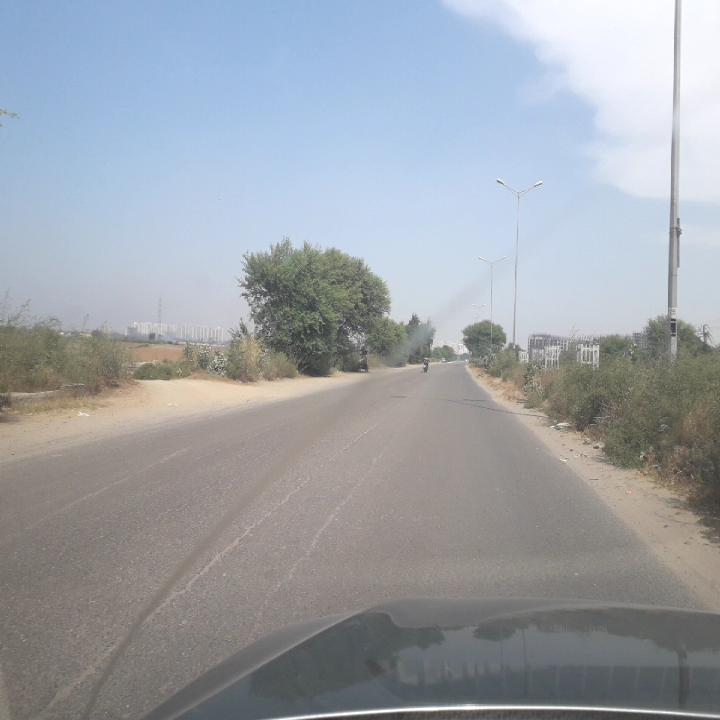
\includegraphics[width=\linewidth,height=3.05cm,keepaspectratio]{assets/longitudinal_crack_1.jpg}\\[3mm]
\textbf{D00}\\Longitudinal crack
\end{column}
\begin{column}{.24\textwidth}\centering
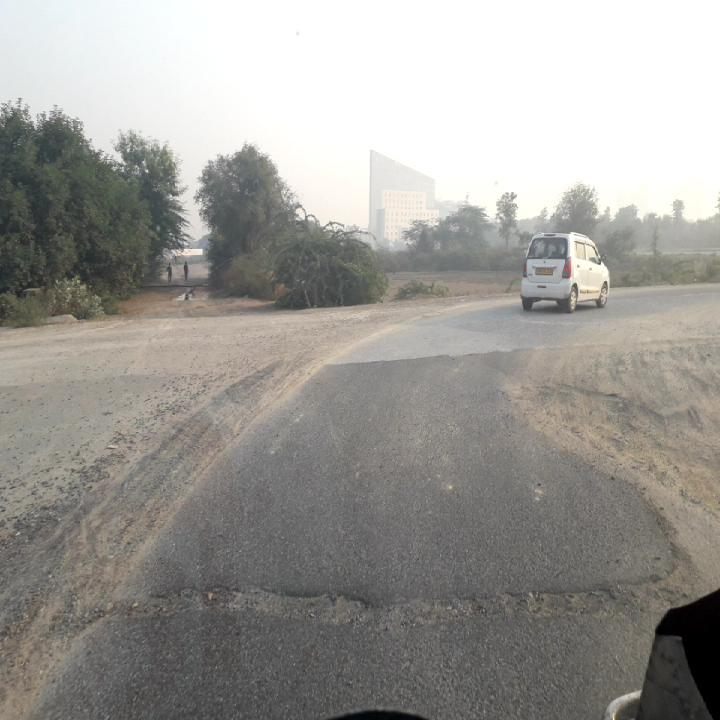
\includegraphics[width=\linewidth,height=3.05cm,keepaspectratio]{assets/transverse_crack_1.jpg}\\[3mm]
\textbf{D10}\\Transverse crack
\end{column}
\begin{column}{.24\textwidth}\centering
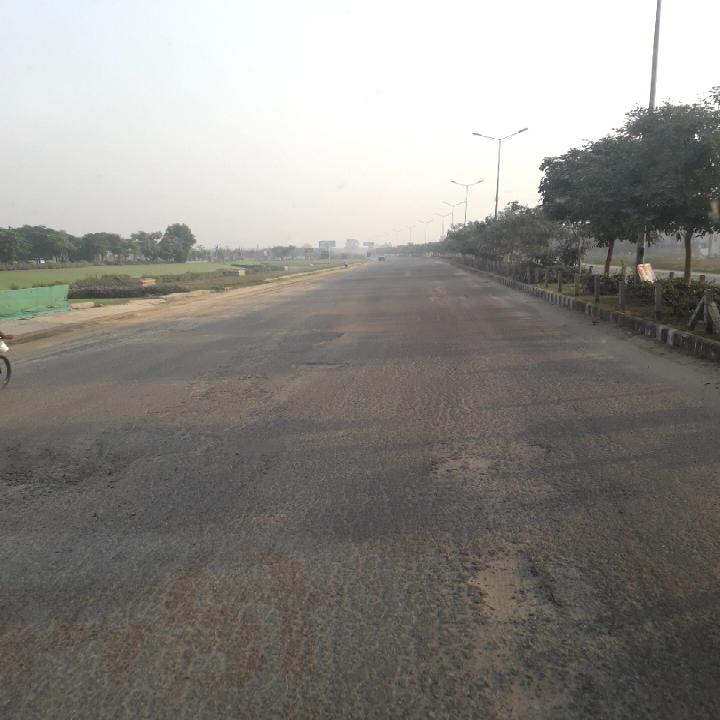
\includegraphics[width=\linewidth,height=3.05cm,keepaspectratio]{assets/alligator_crack_1.jpg}\\[3mm]
\textbf{D20}\\Alligator crack
\end{column}
\begin{column}{.24\textwidth}\centering
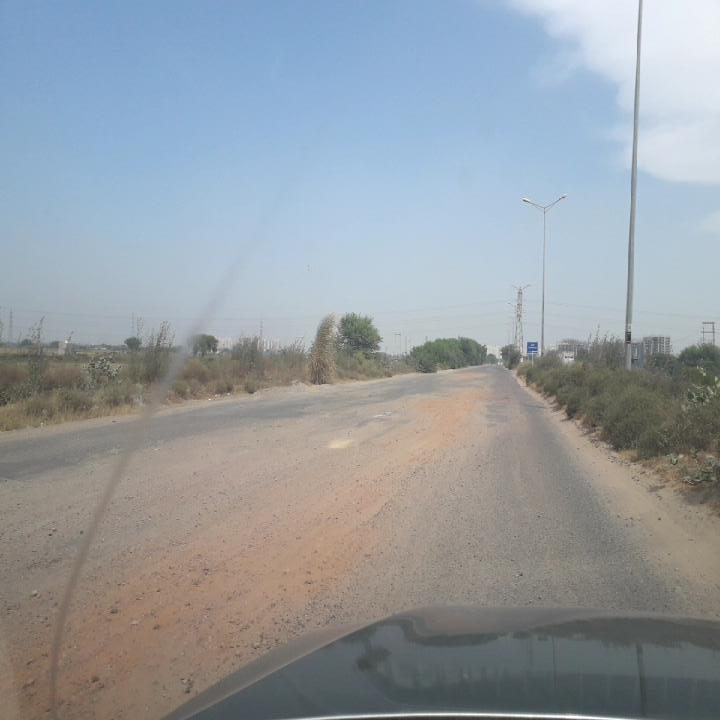
\includegraphics[width=\linewidth,height=3.05cm,keepaspectratio]{assets/pothole_1.jpg}\\[3mm]
\textbf{D40}\\Pothole
\end{column}
\end{columns}
\medskip
\textbf{Task:} predict a bounding box, damage class and confidence for each detected region.
\source{RDD2022 images in local test samples [2]; examples show dataset content, not model predictions.}
\end{frame}

\section{Literature Review}
\begin{frame}{Literature Review}
\small
\renewcommand{\arraystretch}{1.45}
\begin{tabular}{p{2.6cm}p{5cm}p{5.2cm}}
\toprule
\textbf{Work} & \textbf{Contribution} & \textbf{Relevance to this project}\\\midrule
RDD2022 [2] & Road damage images from six countries with four target damage categories. & Common annotation scheme and realistic road scenes.\\
YOLOv8n [3] & Compact, single-stage object detector with multi-scale predictions. & Pretrained baseline for the local prototype.\\
Zeng \& Zhong, 2024 [1] & YOLOv8-PD combines attention, Ghost feature extraction and a shared detection head. & Main reference for the proposed model variants.\\\bottomrule
\end{tabular}
\source{Selected paper [1]; RDD2022 benchmark [2]; pinned Ultralytics implementation [3].}
\end{frame}

\begin{frame}{Literature Review: What YOLOv8-PD Changes}
\small
\renewcommand{\arraystretch}{1.5}
\begin{tabular}{p{2.8cm}p{5cm}p{5cm}}
\toprule\textbf{Component} & \textbf{Purpose in the paper} & \textbf{Intended benefit}\\\midrule
BOT & Add global context through attention. & Relate separated or elongated crack features.\\
LSKA & Use large separable kernels for spatial attention. & Capture a broader region of road texture.\\
C2fGhost & Generate features with cheaper operations. & Reduce feature-extraction cost in the neck.\\
LSCD & Share convolutional detection layers across scales. & Reduce detection-head parameters.\\\bottomrule
\end{tabular}
\medskip
The paper balances detection performance against model size and computation.
\source{Zeng \& Zhong (2024), proposed methodology [1].}
\end{frame}

\section{Identified Gaps}
\begin{frame}{Identified Gaps}
\begin{itemize}\setlength\itemsep{4mm}
\item \textbf{Small and multiple potholes remain difficult.} The reference paper reports missed detections and lower AP for D40.
\item \textbf{Class imbalance limits evaluation.} The local validation set has only nine D10 objects.
\item \textbf{Reproduction needs care.} Some attention and head details are insufficiently specified for an exact replica.
\item \textbf{Comparable evidence is missing locally.} A short baseline run cannot establish the value of individual modifications.
\end{itemize}
\source{Paper discussion [1]; local dataset audit; project architecture notes [4].}
\end{frame}

\section{Problem Statement and Objectives}
\begin{frame}{Problem Statement \& Objectives}
\begin{block}{Problem statement}
Develop an image-based system that localizes and classifies four road damage types, and evaluates detection quality using a reproducible workflow.
\end{block}
\medskip
\begin{enumerate}\setlength\itemsep{3mm}
\item Prepare validated annotations and separate train, validation and test sets.
\item Train and evaluate a pretrained YOLOv8n baseline.
\item Implement and later compare paper-inspired architectural variants.
\item Provide an interface for image upload, detection and result export.
\end{enumerate}
\end{frame}

\section{Proposed Method}
\begin{frame}{Proposed Method: End-to-End Workflow}
\centering
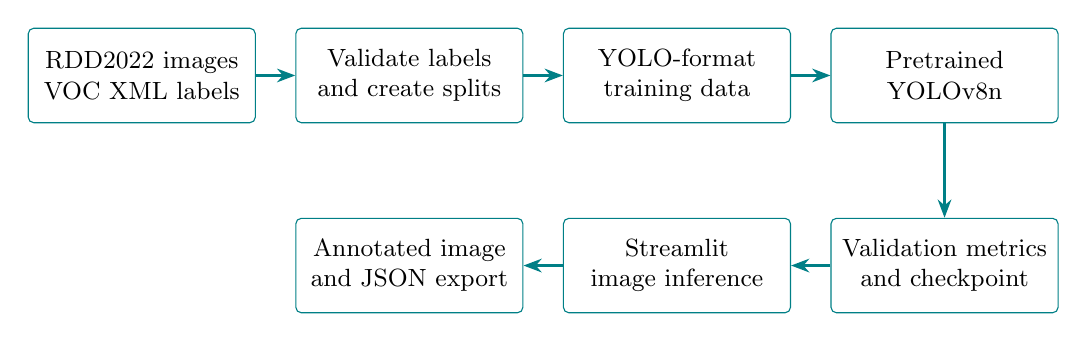
\begin{tikzpicture}[node distance=5mm, every node/.style={font=\small}, box/.style={draw=teal,rounded corners=2pt,align=center,minimum height=12mm,text width=2.65cm}, arr/.style={-{Stealth},thick,teal}]
\node[box] (a) {RDD2022 images\\VOC XML labels};
\node[box,right=of a] (b) {Validate labels\\and create splits};
\node[box,right=of b] (c) {YOLO-format\\training data};
\node[box,right=of c] (d) {Pretrained\\YOLOv8n};
\draw[arr] (a)--(b);\draw[arr] (b)--(c);\draw[arr] (c)--(d);
\node[box,below=12mm of d] (e) {Validation metrics\\and checkpoint};
\node[box,left=of e] (f) {Streamlit\\image inference};
\node[box,left=of f] (g) {Annotated image\\and JSON export};
\draw[arr] (d)--(e);\draw[arr] (e)--(f);\draw[arr] (f)--(g);
\end{tikzpicture}
\par\bigskip\raggedright
\textbf{Implementation:} Python, PyTorch, Ultralytics and Streamlit.\\[2mm]
\textbf{Research extension:} train individual modifications and the combined PD-inspired model under the same protocol.
\source{Local application, training code and architecture documentation [4].}
\end{frame}

\begin{frame}{Proposed Method: Architecture and Implementation Status}
\small
\renewcommand{\arraystretch}{1.4}
\begin{tabular}{p{2.2cm}p{7cm}p{3.6cm}}
\toprule\textbf{Variant} & \textbf{Local implementation} & \textbf{Evidence available}\\\midrule
Baseline & Standard YOLOv8n; four-class detection output. & Three real-data epochs.\\
BOT / LSKA & Residual attention and factorized spatial kernels. & Implemented; smoke checks.\\
Ghost & Replace four neck C2f blocks with C2fGhost. & Implemented; smoke checks.\\
LSCD & Shared GroupNorm head across three scales. & Implemented; smoke checks.\\
PD-inspired & Combine the four modifications. & No local real-data result.\\\bottomrule
\end{tabular}
\medskip
\textbf{Boundary:} these variants are paper-inspired implementations, not an exact reproduction. Their accuracy and efficiency remain to be measured.
\source{docs/architecture.md and local experiment metadata [4].}
\end{frame}

\begin{frame}{Proposed Method: Dataset Preparation}\small
\begin{columns}[T]
\begin{column}{.53\textwidth}
\lead{6,650 retained India images}
\begin{itemize}\setlength\itemsep{3mm}
\item Convert VOC XML boxes to normalized YOLO coordinates.
\item Check labels, image dimensions and bounding boxes.
\item Skip 1,056 images containing unsupported classes, including D44.
\item Check exact image duplicates before splitting.
\end{itemize}
\end{column}
\begin{column}{.42\textwidth}
\renewcommand{\arraystretch}{1.5}
\begin{tabular}{lrr}\toprule
\textbf{Split}&\textbf{Images}&\textbf{Share}\\\midrule
Train&5,320&80\%\\
Validation&665&10\%\\
Test&665&10\%\\\bottomrule
\end{tabular}
\medskip\par
\small Seed: 42. No exact duplicates found.\\[2mm]
Sequence grouping was not used; nearby frames may still be correlated.
\end{column}
\end{columns}
\source{Local split manifest and dataset audit [4]. Test set reserved; no held-out test score reported.}
\end{frame}

\section{Experimental Result and Analysis}
\begin{frame}{Experimental Setup: Two Different Protocols}
\small\renewcommand{\arraystretch}{1.4}
\begin{tabular}{p{3.2cm}p{4.7cm}p{4.8cm}}
\toprule &\textbf{Reference paper [1]}&\textbf{Local baseline [4]}\\\midrule
Data & 10,000 selected images; six countries & 6,650 retained India images\\
Train / validation & 8,000 / 2,000 & 5,320 / 665; 665 reserved for test\\
Epochs / batch & 300 / 16 & 3 / 4\\
Input size & $640\times640$ & $640\times640$\\
Optimizer / initial LR & SGD / 0.01 & SGD / 0.01\\
Compute & NVIDIA RTX 2060, 6 GB & CPU\\
Model & YOLOv8n and YOLOv8-PD & Pretrained YOLOv8n baseline\\\bottomrule
\end{tabular}
\medskip
\textbf{Interpretation:} the two results are contextual references, not a controlled head-to-head comparison.
\end{frame}

\begin{frame}{Evaluation Metrics}
\begin{columns}[T]
\begin{column}{.48\textwidth}
\lead{Detection quality}
\[\mathrm{Precision}=\frac{TP}{TP+FP}\] \[
\mathrm{Recall}=\frac{TP}{TP+FN}\]
\small
Precision measures how many predictions are correct. Recall measures how many annotated objects are recovered.\\[3mm]
A detection must match both the class and the required box overlap.
\end{column}
\begin{column}{.48\textwidth}
\lead{Localization and efficiency}
\small
\textbf{IoU:} intersection area divided by union area of predicted and reference boxes.\\[3mm]
\textbf{mAP@0.50:} mean average precision across classes at IoU 0.50.\\[3mm]
\textbf{mAP@0.50:0.95:} average across IoU thresholds 0.50--0.95; stricter localization.\\[3mm]
\textbf{Parameters / GFLOPs:} model size and computational cost.
\end{column}
\end{columns}
\source{Metric definitions used in the reference paper and Ultralytics evaluation [1,3].}
\end{frame}

\begin{frame}{Published Results: YOLOv8-PD}
\centering\renewcommand{\arraystretch}{1.55}
\begin{tabular}{lrrr}\toprule
\textbf{Metric}&\textbf{YOLOv8n}&\textbf{YOLOv8-PD}&\textbf{Change}\\\midrule
mAP@0.50&69.2\%&70.6\%&+1.4 pp\\
mAP@0.50:0.95&38.0\%&39.5\%&+1.5 pp\\
F1 score&0.67&0.68&+0.01\\
Parameters&3.1 M&2.3 M&$\approx$25.8\% fewer\\
GFLOPs&8.2&6.1&$\approx$25.6\% fewer\\\bottomrule
\end{tabular}
\par\bigskip\raggedright
\textbf{Published finding:} a modest detection improvement with lower model cost. These are the authors' results, not results achieved by this project.
\source{Zeng \& Zhong (2024), Tables 1 and 5 [1]. Reductions calculated from rounded table values; pp = percentage points.}
\end{frame}

\begin{frame}{Local Results: Preliminary Three-Epoch Baseline}
\begin{columns}[T]
\begin{column}{.46\textwidth}
\lead{Final-epoch validation}
\renewcommand{\arraystretch}{1.55}
\begin{tabular}{lr}\toprule
Precision&\textbf{37.92\%}\\
Recall&\textbf{12.30\%}\\
mAP@0.50&\textbf{8.33\%}\\
mAP@0.50:0.95&\textbf{3.16\%}\\\bottomrule
\end{tabular}
\end{column}
\begin{column}{.49\textwidth}
\lead{Validation trend}
\small\renewcommand{\arraystretch}{1.55}
\begin{tabular}{rrr}\toprule
\textbf{Epoch}&\textbf{mAP@.50}&\textbf{mAP@.50:.95}\\\midrule
1&2.27\%&0.82\%\\
2&5.36\%&1.91\%\\
3&8.33\%&3.16\%\\\bottomrule
\end{tabular}
\medskip\par
Improvement across three epochs is encouraging, but does not establish convergence or reliable detection.
\end{column}
\end{columns}
\source{runs/train/first\_model2/results.csv, epochs 1--3 [4]. These are validation log values, not a separate best-checkpoint test evaluation.}
\end{frame}

\begin{frame}{Analysis: Imbalance and Limited Training}\small
\begin{columns}[T]
\begin{column}{.45\textwidth}
\small\renewcommand{\arraystretch}{1.55}
\begin{tabular}{lrrr}\toprule
\textbf{Objects}&\textbf{Train}&\textbf{Val.}&\textbf{Test}\\\midrule
D00&1,118&141&160\\
D10&50&9&4\\
D20&1,313&154&168\\
D40&2,403&279&274\\\bottomrule
\end{tabular}
\medskip\par
D10 accounts for only about \textbf{1\%} of training objects.
\end{column}
\begin{column}{.51\textwidth}
\begin{itemize}\setlength\itemsep{3mm}
\item Low recall indicates many objects remain undetected.
\item Three epochs do not establish convergence.
\item Few D10 examples make evaluation unstable.
\item Longer training and matched experiments are needed for comparison.
\end{itemize}
\end{column}
\end{columns}
\source{Local audit and validation logs [4]. Causes require further experiments.}
\end{frame}

\section{Conclusion and Future Work}
\begin{frame}{Conclusion and Future Work}\small
\begin{columns}[T]
\begin{column}{.47\textwidth}
\lead{Completed}
\begin{itemize}\setlength\itemsep{3mm}
\item Validated dataset conversion and reproducible split preparation.
\item Local baseline training with recorded validation metrics.
\item Image upload, detection, statistics and export interface.
\item Paper-inspired variants available for further experiments.
\end{itemize}
\end{column}
\begin{column}{.48\textwidth}
\lead{Next experiments}
\begin{itemize}\setlength\itemsep{3mm}
\item Train to convergence with checkpoint recovery.
\item Improve rare-class coverage; assess sequence-aware splits.
\item Compare baseline, each module and the combined model with matched settings.
\item Evaluate the held-out test set, efficiency and failure cases.
\end{itemize}
\end{column}
\end{columns}
\medskip
\textbf{Current conclusion:} the prototype works as an experimental pipeline; improved accuracy over the paper has not been demonstrated.
\end{frame}

\section{Publications}
\begin{frame}{Publications (if any)}
\lead{No project publication has been reported at this stage.}
\bigskip
The selected Scientific Reports article is a reference publication by Jiayi Zeng and Han Zhong; it is not a publication from this project.
\bigskip
\begin{block}{Before preparing a research submission}
Complete controlled experiments, document implementation differences, evaluate the held-out test set and report reproducible results.
\end{block}
\end{frame}

\section{References}
\begin{frame}{References}
\small
\begin{enumerate}\setlength\itemsep{4mm}
\item J. Zeng and H. Zhong, ``YOLOv8-PD: an improved road damage detection algorithm based on YOLOv8n model,'' \textit{Scientific Reports}, vol. 14, article 12052, 2024.\\
\href{https://doi.org/10.1038/s41598-024-62933-z}{doi:10.1038/s41598-024-62933-z}.
\item RDD2022 dataset and Global Road Damage Detection Challenge resources.\\
\url{https://github.com/sekilab/RoadDamageDetector}
\item Ultralytics, YOLOv8 implementation. Local project version: 8.3.203.\\
\url{https://github.com/ultralytics/ultralytics/tree/v8.3.203}
\item Project evidence: dataset audit, split manifest, architecture notes and local run \texttt{first\_model2} (experiment metadata, arguments and results CSV).
\end{enumerate}
\source{Institute logo: official NIT Patna website, \url{https://www.nitp.ac.in/}. Detailed asset and result provenance is included with the source files.}
\end{frame}
\end{document}
